\section{Analysis}
\label{sec:analysis}

The experiments fix the system; this section explains why it looks the way it does, and is
careful to separate what we can measure from what we can only describe.
Section~\ref{sec:val_lb} documents the central decoupling of the project: held-out accuracy on
the single-plant validation split barely predicts multi-species quadrat Macro F1, which reframes
the bottleneck as a distribution-shift problem rather than a model-capacity one.
Section~\ref{sec:head_repr} probes the trained head representations with linear CKA and
taxonomic-separation diagnostics; this analysis is \emph{descriptive}, not causal.
Section~\ref{sec:orthogonality} shows that variants within our own backbone have saturated into
essentially one model, which both motivated the search for orthogonal evidence sources and
explains its failure. Section~\ref{sec:longtail} examines why flattening the long tail hurt rather
than helped.

\subsection{Validation vs Leaderboard Mismatch}
\label{sec:val_lb}

A striking decoupling runs through every model-selection decision in this project: held-out
accuracy on the single-plant distribution barely predicts Macro F1 on the multi-species quadrat
leaderboard. Across our twelve strongest runs the two metrics correlate at only $r \approx 0.4$
(Figure~\ref{fig:val_vs_kaggle}), and within the unfrozen-blocks ablation of
Table~\ref{tab:blocks} they invert outright: validation top-5 accuracy rises monotonically with
unfrozen capacity while leaderboard Macro F1 peaks in the middle and collapses at full
fine-tune. We read this as direct evidence that the bottleneck on this benchmark is the
single-plant to multi-species distribution shift, not model capacity on the single-plant
distribution itself. It is also why we use validation accuracy only to choose checkpoints, never
to rank final submissions (\S\ref{sec:eval_protocol}): the headline anchor does not sit at the
validation maximum, and the configurations that do (the i003 capped checkpoints, the 015
PlantCLEF24+iNaturalist mix) score lower on the leaderboard.

\begin{figure}[!htbp]
  \centering
  % Chart C: Validation top-5 vs Kaggle Macro F1 across our twelve strongest runs.
% Source: chart_data.js VAL_VS_KAGGLE.
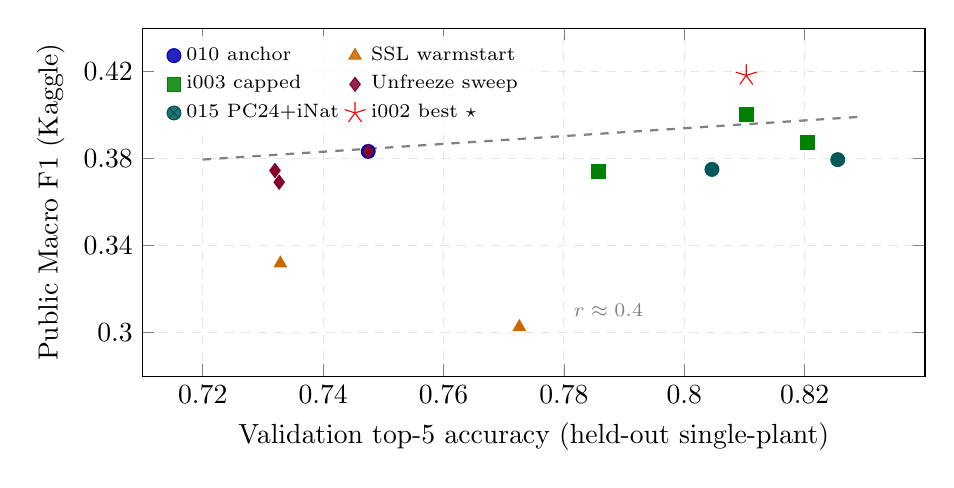
\begin{tikzpicture}
  \begin{axis}[
      width=0.95\linewidth, height=6.0cm,
      xlabel={Validation top-5 accuracy (held-out single-plant)},
      ylabel={Public Macro F1 (Kaggle)},
      xmin=0.71, xmax=0.84,
      ymin=0.28, ymax=0.44,
      xtick={0.72,0.74,0.76,0.78,0.80,0.82},
      ytick={0.30,0.34,0.38,0.42},
      grid=major, grid style={dashed,gray!20},
      legend style={at={(0.02,0.98)}, anchor=north west,
                    font=\scriptsize, draw=none, fill=white,
                    fill opacity=0.85, text opacity=1,
                    cells={anchor=west}},
      legend columns=2,
      ylabel near ticks,
      xlabel near ticks,
      scatter/classes={
        ours={mark=*,blue!70!black},
        ssl={mark=triangle*,orange!80!black},
        cap={mark=square*,green!50!black},
        sweep={mark=diamond*,purple!70!black},
        inat={mark=otimes*,teal!70!black},
        best={mark=star,red,mark size=4pt}
      },
    ]
    \addplot[scatter, only marks, mark size=2.5pt,
             scatter src=explicit symbolic]
      table[meta=label] {
        x       y        label
        0.7475  0.38333  ours
        0.7726  0.30261  ssl
        0.7329  0.33185  ssl
        0.7858  0.37421  cap
        0.8103  0.40041  cap
        0.8204  0.38761  cap
        0.7320  0.37455  sweep
        0.7475  0.38333  sweep
        0.7327  0.36919  sweep
        0.8046  0.37506  inat
        0.8255  0.37956  inat
        0.8103  0.41826  best
      };
    \legend{010 anchor, SSL warmstart, i003 capped, Unfreeze sweep, 015 PC24+iNat, i002 best $\star$}
    % Spearman fit line (illustrative, r approx 0.4)
    \addplot[gray, dashed, thick, domain=0.72:0.83] {0.25 + 0.18*x};
    \node[font=\scriptsize, gray, anchor=west]
      at (axis cs:0.78,0.31) {$r \approx 0.4$};
  \end{axis}
\end{tikzpicture}

  \caption{Validation top-5 accuracy on the held-out single-plant split versus public Macro F1 on the multi-species quadrat leaderboard, across our twelve strongest runs. The headline anchor ($\star$, i002 last-four-blocks 224+336+LA ensemble) does not sit at the maximum validation point; the i003 capped checkpoints (green squares) and the 015 PC24+iNat mix (teal) reach higher validation accuracy but lower leaderboard score. The dashed line indicates the weak monotone trend ($r \approx 0.4$).}
  \label{fig:val_vs_kaggle}
\end{figure}

\subsection{Head Design and Representation Geometry}
\label{sec:head_repr}

The two supervised fine tunes wire their classification heads differently
(Figure~\ref{fig:head_design}): experiment~010 feeds a single shared multi layer perceptron into
five linear heads, whereas experiment~i002 gives each of its three heads an independent
perceptron. To understand what each design does to the feature space we ran a descriptive probe
of the trained representations. This analysis is not causal: the two experiments also differ in
training data, schedule, number of unfrozen blocks, and head count, and they use different
validation splits, so we compare each representation only against its own encoder and never
compute cross experiment similarity (only $62$ of the $4{,}000$ sampled images overlap between
the two splits).

For a family stratified sample of $4{,}000$ validation images per experiment we captured the
BioCLIP encoder feature and every MLP hidden vector with forward hooks, then measured linear
centred kernel alignment (CKA) and lightweight taxonomic separation diagnostics (cosine
silhouette at the genus and family levels). The results are summarised in
Table~\ref{tab:head_repr} and Figure~\ref{fig:head_taxstruct}.

Two observations are robust within each experiment. First, every MLP output stays highly aligned
with its own encoder feature (linear CKA between $0.75$ and $0.84$), so neither head design
discards the BioCLIP geometry. In i002 the three per head MLPs are distinct rather than redundant
copies (pairwise CKA $0.73$ to $0.84$): the family MLP departs most from both the encoder
($0.75$) and the species MLP ($0.73$), while the species MLP stays closest to the encoder
($0.82$). Second, in both designs the trained MLP is modestly more taxonomically structured than
that experiment's own raw encoder feature (for example the 010 shared trunk raises genus cosine
silhouette from $0.18$ to $0.21$). Within i002 the genus and family MLPs separate taxa more
sharply than the species MLP (family level silhouette $0.26$ for the family MLP versus $0.16$ for
the species MLP), which is the expected signature of each MLP specialising toward its own head's
loss.

We stress that these are descriptive statements about representation geometry. They characterise
what the shared and per head designs do to the feature space, but they do not isolate the effect
of the head topology on the leaderboard score, which remains confounded with the data and
schedule differences between the two experiments. We therefore make no causal claim, and we do
not treat the 010 versus i002 comparison as a controlled ablation.

\begin{table}[ht]
  \centering
  \small
  \setlength{\tabcolsep}{4pt}
  \begin{tabular}{@{}llccc@{}}
    \toprule
    Exp. & Representation & CKA$\to$enc. & Fam.\ silh. & Gen.\ silh. \\
    \midrule
    010  & encoder       & ---    & 0.134 & 0.183 \\
    010  & shared MLP    & 0.845  & 0.177 & 0.215 \\
    \cmidrule(lr){1-5}
    i002 & encoder       & ---    & 0.134 & 0.185 \\
    i002 & species MLP   & 0.821  & 0.158 & 0.220 \\
    i002 & genus MLP     & 0.806  & 0.193 & 0.252 \\
    i002 & family MLP    & 0.749  & 0.260 & 0.296 \\
    \bottomrule
  \end{tabular}
  \caption{Within experiment representation analysis. CKA is linear centred kernel alignment of each MLP output to its own encoder feature; silhouette is cosine, at the family and genus levels, on the same $4{,}000$-image sample. Cross experiment CKA is omitted because the two experiments use different validation splits (only $62/4{,}000$ sampled images overlap). i002 cross head CKA: species/genus $0.84$, species/family $0.73$, genus/family $0.84$.}
  \label{tab:head_repr}
\end{table}

\begin{figure}[!htbp]
  \centering
  % Taxonomy-structure bars -- cosine silhouette per head representation, family
% and genus levels. Within-experiment only (see caption).
% Source: report/head_features/tex_plan/taxonomy_structure_plot_data.csv
%   (== tex_info/taxonomy_structure_metrics.csv / plot_data_for_tex.csv silhouette_*).
% Style follows figures/unfreeze_sweep.tex. Include in a single-column figure.
\begin{tikzpicture}
  \begin{groupplot}[
      group style={group size=2 by 1, horizontal sep=1.5cm},
      width=5.0cm, height=5.0cm,
      ymin=0, ymax=0.33,
      ytick={0,0.1,0.2,0.3},
      ylabel near ticks,
      symbolic x coords={010 enc, 010 shr, i02 enc, i02 sp, i02 ge, i02 fa},
      xtick=data,
      xticklabel style={rotate=55, anchor=east, font=\tiny},
      yticklabel style={font=\scriptsize},
      grid=major, grid style={dashed,gray!20},
      enlarge x limits=0.10,
      every node near coord/.append style={font=\tiny, color=black!70},
    ]
    % ---- Family-level silhouette ----
    \nextgroupplot[ybar, bar width=7pt, title={Family-level}, title style={font=\small}, ylabel={Cosine silhouette}]
      \addplot+[draw=blue!55!black, fill=blue!28]
        coordinates {(010 enc,0.1343) (010 shr,0.1766) (i02 enc,0.1336)
                     (i02 sp,0.1579) (i02 ge,0.1928) (i02 fa,0.2597)};
      \node[anchor=south, font=\tiny, color=orange!75!black] at (axis cs:i02 fa,0.2597) {0.26};

    % ---- Genus-level silhouette ----
    \nextgroupplot[ybar, bar width=7pt, title={Genus-level}, title style={font=\small}]
      \addplot+[draw=blue!55!black, fill=blue!28]
        coordinates {(010 enc,0.1829) (010 shr,0.2148) (i02 enc,0.1851)
                     (i02 sp,0.2200) (i02 ge,0.2517) (i02 fa,0.2958)};
      \node[anchor=south, font=\tiny, color=orange!75!black] at (axis cs:i02 fa,0.2958) {0.30};
  \end{groupplot}
\end{tikzpicture}

  \caption{Taxonomic structure of each head representation on the family stratified $4{,}000$-image samples: cosine silhouette at the family and genus levels. Within each experiment the trained MLP increases structure over its own raw encoder feature; within i002 the family and genus MLPs are the most structured (family level silhouette $0.26$ for the family MLP versus $0.16$ for the species MLP). Magnitudes are comparable only within an experiment, not across, because the two experiments use different validation samples.}
  \label{fig:head_taxstruct}
\end{figure}

\subsection{Within-backbone Saturation and Orthogonality}
\label{sec:orthogonality}

Before pivoting to architecture-orthogonal evidence sources, we measured whether further
within-backbone diversity could break the i002 anchor by comparing the four-blocks i002
checkpoint against the eight-blocks i002 checkpoint and against epoch-5 versions of both.
Table~\ref{tab:within} reports the pairwise top-one agreement and submission Jaccard on $2{,}105$
test quadrats.

\begin{table}[ht]
  \centering
  \small
  \setlength{\tabcolsep}{2pt}
  \begin{tabular}{@{}p{0.48\linewidth}cc@{}}
    \toprule
    Pair & Top-1 & Jaccard \\
    \midrule
    blk\_4 vs.\ blk\_8 & 0.901 & --- \\
    blk\_4 vs.\ blk\_4 (epoch 5) & 0.807 & 0.664 \\
    4-way intra-BC2.5 ens.\ vs.\ anchor & --- & 0.923 \\
    \bottomrule
  \end{tabular}
  \caption{Within-backbone diagnostic gates. Top-1 agreement on a 7{,}806-way classifier and submission Jaccard at the operating threshold.}
  \label{tab:within}
\end{table}

The $0.923$ Jaccard between the four-way intra-BioCLIP~2.5 ensemble and our anchor submission
shows that all within-backbone variants are essentially one model on the test set: shuffling the
unfrozen depth or the training-epoch index does not move the prediction distribution. This is
what motivated the three architecture-orthogonal pivots (\S\ref{sec:final_results}): if the
remaining headroom is not inside the backbone, it must come from a signal the backbone cannot
read.

The pivots' near-zero deltas (Table~\ref{tab:summary}) reveal an under-appreciated property of
strong fine-tuned visual classifiers on biological data: \emph{information-theoretic
orthogonality is not the same as statistical orthogonality} once the visual model has been
trained on data where the auxiliary signal is naturally correlated with image content. cRT was
structurally orthogonal but introduced wrong evidence and dragged the anchor down by $0.036$;
genus reweighting was statistically dependent on the BioCLIP~2.5 posterior itself and moved the
score by $-0.006$, close to the noise floor; the seasonal phenology prior, the most genuinely
orthogonal source we tested (since date is not in the image at all), moved the score by only
$-0.005$, again close to the noise floor, because the seasonal structure was already implicit in
the leaf and flower phenotypes seen during training. The practical reading is that real headroom
on this benchmark requires structurally stronger \emph{visual} models rather than post hoc
reweighting with auxiliary priors (\S\ref{sec:discussion}).

\subsection{Long-tail Behaviour}
\label{sec:longtail}

The cleanest near-controlled counterfactual in the project concerns the long tail. Experiment
i003 takes the i002 manifest, augments the tail with $148{,}063$ GBIF-sourced images
(of $161{,}686$ candidates, after dropping $13{,}623$ that failed image decoding) for the
$2{,}020$ species with fewer than one hundred training examples, and then caps every species at
five hundred images, flattening the head of the distribution (Figure~\ref{fig:long_tail}).
Because i003 changes only the training manifest relative to i002, the leaderboard outcome is
unusually interpretable, and it is a surprise: this flatter distribution \emph{hurt}, with the
i003 best reaching $0.40041$ public Macro F1 against $0.41826$ for the corresponding uncapped
i002 checkpoint. We read this as direct evidence that, on this benchmark, the marginal value of
additional head-class examples is positive provided their label quality is high: capping discards
information rather than rebalancing it. The augmentation did not lift any species above the
hundred-image floor, so the long tail itself remained long (Figure~\ref{fig:long_tail}, left
bins); the cap only trimmed the head. Full manifest statistics are given in
Appendix~\ref{sec:cap_extra_detail}.

\begin{figure}[!htbp]
  \centering
  % Chart F: Species long-tail before vs after 500-cap (i003 manifest).
% Source: chart_data.js SPECIES_LONG_TAIL.
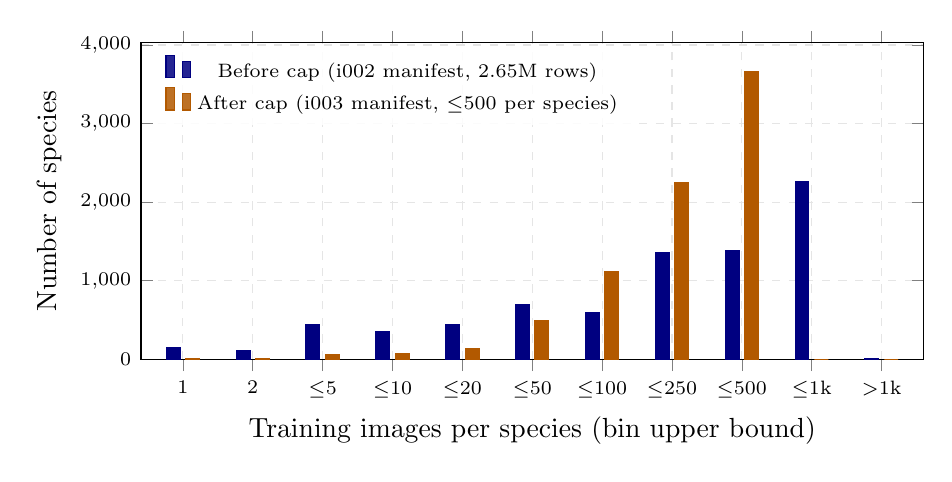
\begin{tikzpicture}
  \begin{axis}[
      width=0.95\linewidth, height=5.6cm,
      ybar=2pt,
      bar width=5pt,
      enlarge x limits=0.06,
      ymin=0,
      ylabel={Number of species},
      xlabel={Training images per species (bin upper bound)},
      symbolic x coords={1,2,$\le$5,$\le$10,$\le$20,$\le$50,$\le$100,$\le$250,$\le$500,$\le$1k,$>$1k},
      xtick=data,
      xticklabel style={font=\scriptsize, rotate=0},
      yticklabel style={font=\scriptsize},
      ylabel near ticks,
      legend style={at={(0.02,0.98)}, anchor=north west,
                    font=\scriptsize, draw=none, fill=white,
                    fill opacity=0.85, text opacity=1},
      grid=major, grid style={dashed,gray!20},
      nodes near coords={},
    ]
    \addplot+[fill=blue!50!black, draw=blue!50!black]
      coordinates {
        (1,145) (2,109) ($\le$5,445) ($\le$10,349) ($\le$20,445)
        ($\le$50,698) ($\le$100,595) ($\le$250,1358) ($\le$500,1387)
        ($\le$1k,2263) ($>$1k,12)
      };
    \addlegendentry{Before cap (i002 manifest, 2.65M rows)}
    \addplot+[fill=orange!70!black, draw=orange!70!black]
      coordinates {
        (1,8) (2,9) ($\le$5,58) ($\le$10,71) ($\le$20,138)
        ($\le$50,496) ($\le$100,1120) ($\le$250,2244) ($\le$500,3662)
        ($\le$1k,0) ($>$1k,0)
      };
    \addlegendentry{After cap (i003 manifest, $\le$500 per species)}
  \end{axis}
\end{tikzpicture}

  \caption{Species count per training-image bin, before and after the i003 per-species cap at $500$. The cap collapses the two heaviest bins ($\le$1k and $>$1k) into the $\le$500 bin and lifts middle bins, but does not move species out of the long tail (left bins). This flatter distribution \emph{hurt} the public Macro F1.}
  \label{fig:long_tail}
\end{figure}
